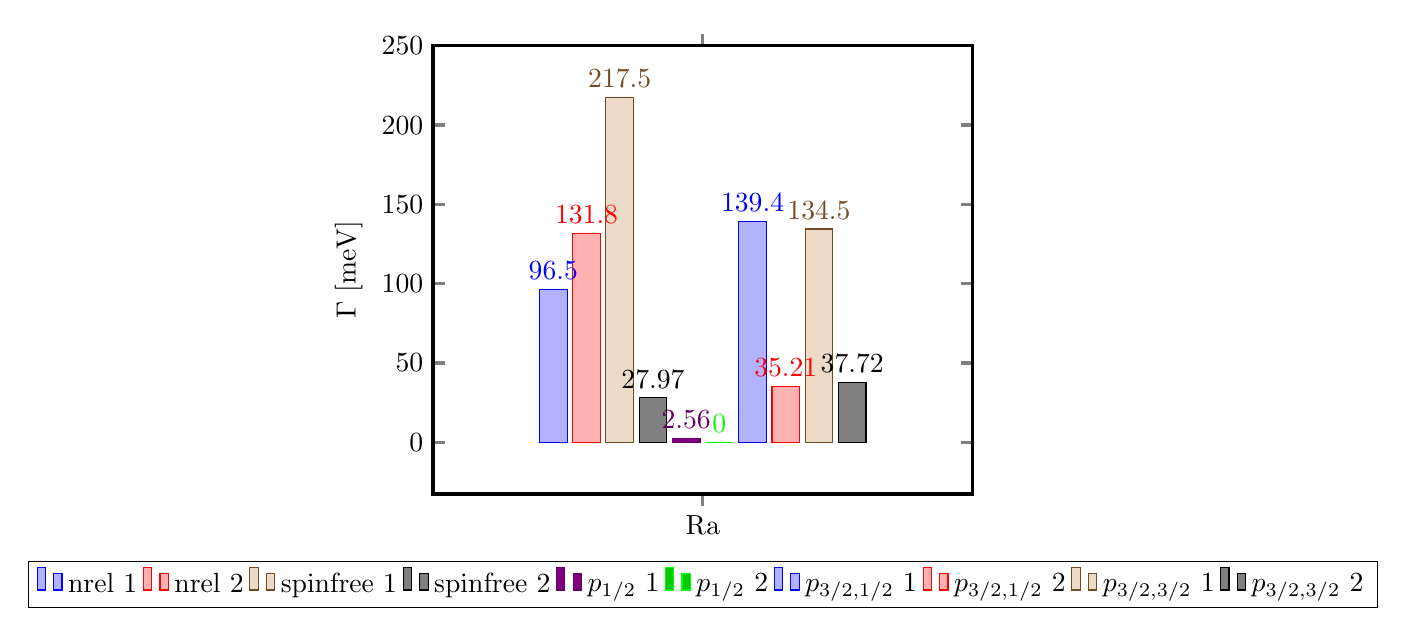
\begin{tikzpicture}
\begin{axis}[
    ybar,
    enlargelimits=0.15,
    legend style={at={(0.5,-0.15)},
      anchor=north,legend columns=-1},
    ylabel={$\Gamma$ [meV]},
    %ylabel={\#participants},
    symbolic x coords={Ra},
    xtick=data,
    nodes near coords,
    nodes near coords align={vertical},
    enlarge x limits=0.25, %space left and right
    axis line style = very thick,
    tick style = very thick
    ]
\addplot coordinates {(Ra,96.50)};
\addplot coordinates {(Ra,131.8)};
\addplot coordinates {(Ra,217.5)};
\addplot coordinates {(Ra,27.97)};
\addplot coordinates {(Ra,2.564)};
\addplot coordinates {(Ra,0)};
\addplot coordinates {(Ra,139.4)};
\addplot coordinates {(Ra,35.21)};
\addplot coordinates {(Ra,134.5)};
\addplot coordinates {(Ra,37.72)};
\legend{nrel 1,nrel 2,spinfree 1,spinfree 2,$p_{1/2}$ 1,$p_{1/2}$ 2,$p_{3/2,1/2}$ 1,$p_{3/2,1/2}$ 2,$p_{3/2,3/2}$ 1,$p_{3/2,3/2}$ 2};
\end{axis}
\end{tikzpicture}

